\documentclass[tikz]{standalone}
\usetikzlibrary{decorations.markings}
\begin{document}
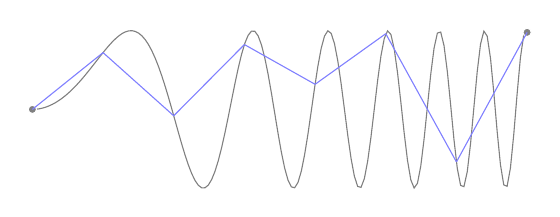
\begin{tikzpicture}[domain=0:6.2832]%[scale=.75,decoration={
%    markings,
%    mark=at position 0.5 with {\arrow{>}}}]
%\draw[black!40,tension=1,] plot [smooth] coordinates {(-1,0) (-1,-.5) (0,-.2) (1,.5) (1,0)};
\draw[gray,samples=150] plot (\x,{sin((\x)^2 r)});
\fill[gray,draw=white] (0,0) circle (1.5pt);
\fill[gray,draw=white] (6.2832,{sin((6.2832)^2 r)}) circle (1.5pt);
\newcommand{\NN}{7}
\foreach \n in {0,...,6}
{
	\draw[blue!50!white] ({6.2832*\n/\NN},{(sin(((6.2832*\n/\NN))^2 r))}) -- ({6.2832*(\n+1)/\NN},{sin( ((6.2832*(\n+1)/\NN))^2 r)});
}
\end{tikzpicture}
\end{document}


